\documentclass[../main.tex]{subfiles}

\begin{document}

We can use "The World \& The Machine" model by M. Jackson and P. Zave to make an initial domain analysis. This allows us to understand which are the entities and the phenomena the machine cannot directly observe ("The World"), which are the ones the external world cannot directly see ("The Machine"), and the ones that are shared, i.e. the mean of interaction between the two.

\begin{figure}[h!]
	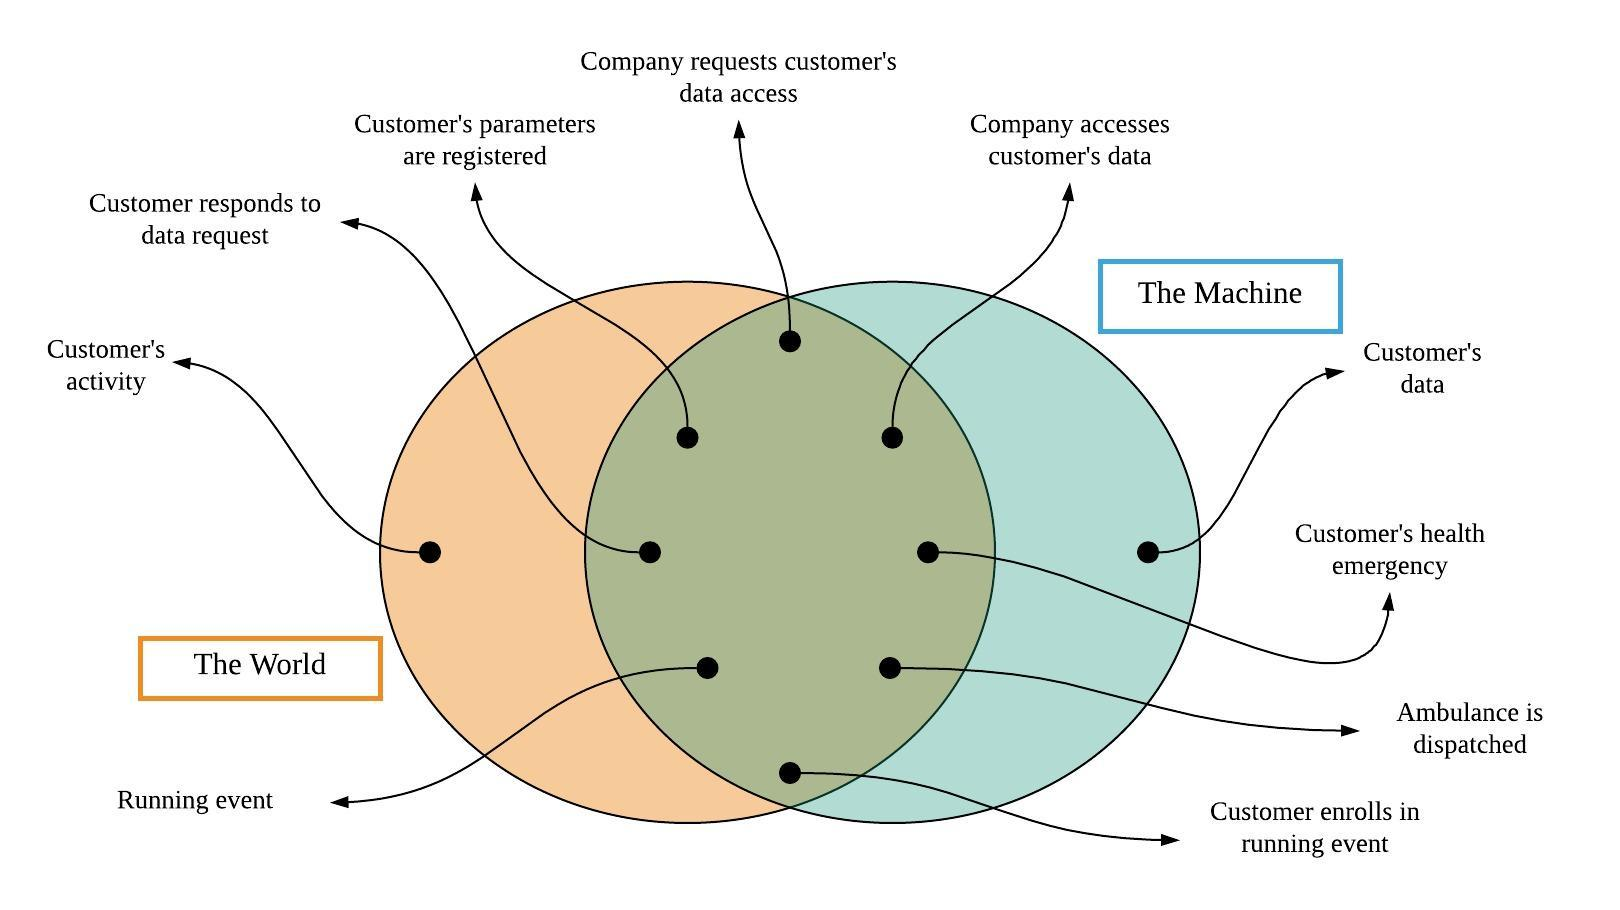
\includegraphics[width=\linewidth]{rasd_worldmachine.jpg}
	\caption{Program analysis as per "The World \& The Machine" model}
	\label{fig:rasd_worldmachine}
\end{figure}

\subsection{Product perspective}

\subsubsection{Class diagrams}

Following there are the class diagrams that give an overall description of our main three services through the use of a conceptual model. Only the relevant parts of the system are present in every one of them for the sake of clarity, but it is to be considered as a single model.
\newpage
\thispagestyle{empty} % to hide page numbers
\begin{figure}[H]
	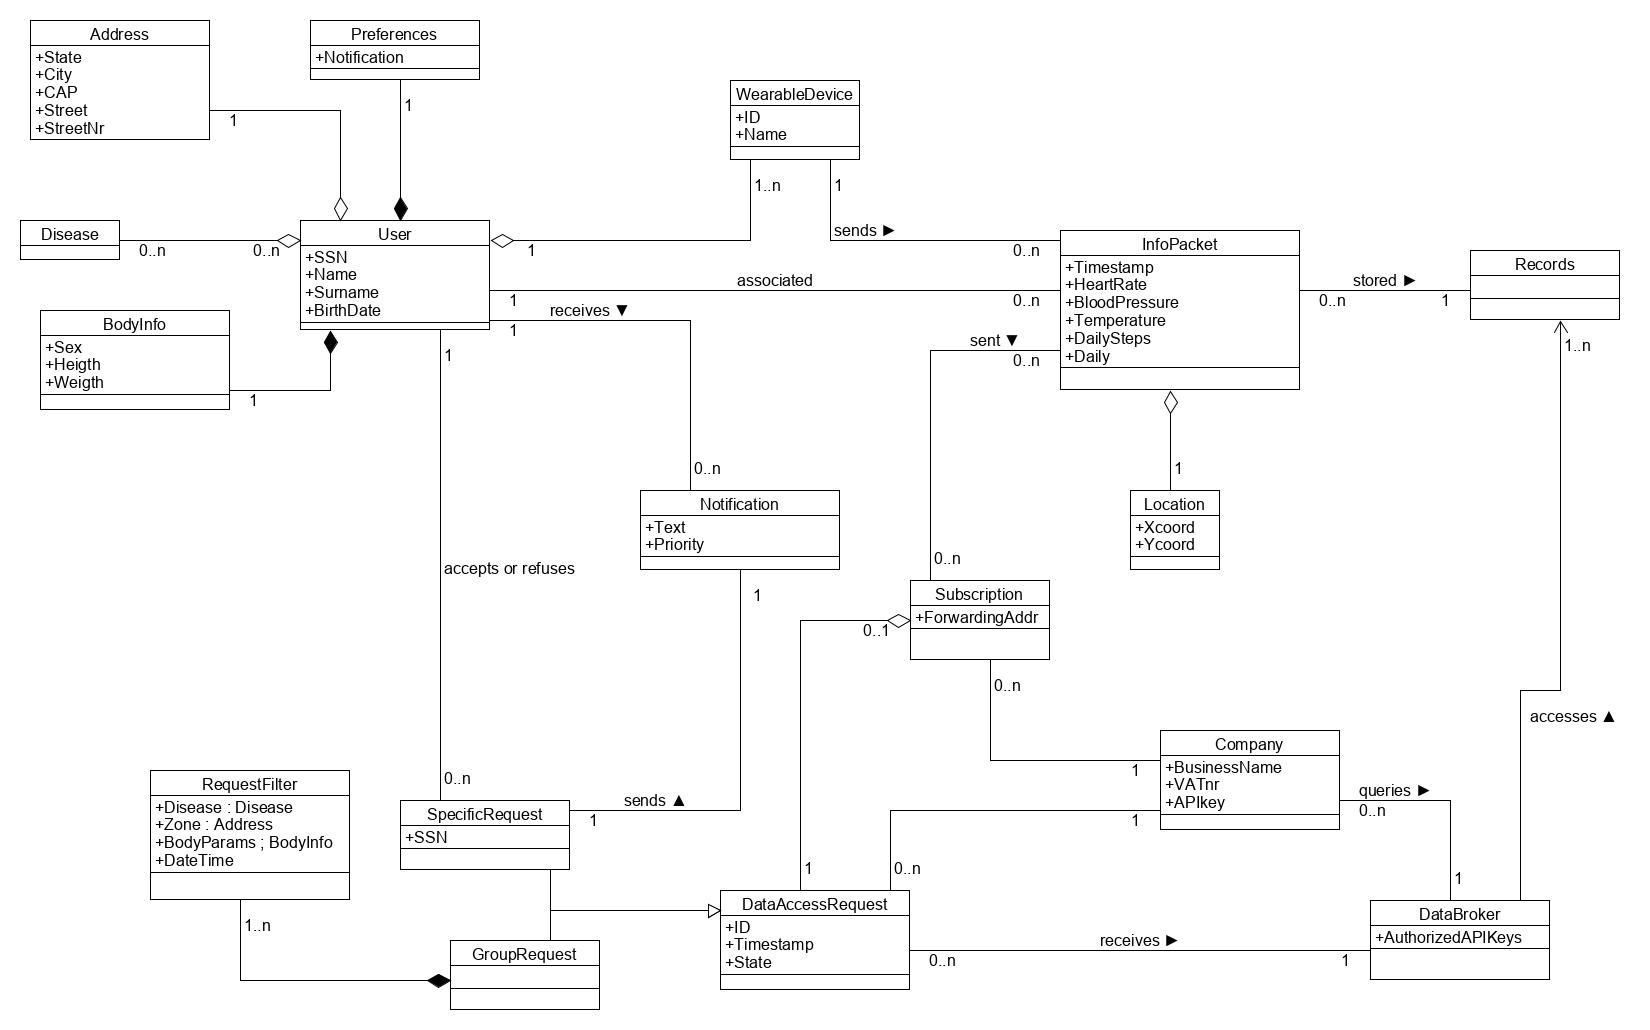
\includegraphics[width=\paperwidth, angle=90]{rasd_classdiag_d4h.jpg}
	\caption{Class diagram for the Data4Help service}
	\label{fig:classdiag_d4h}
\end{figure}
\newpage
\thispagestyle{empty}
\begin{figure}[H]
	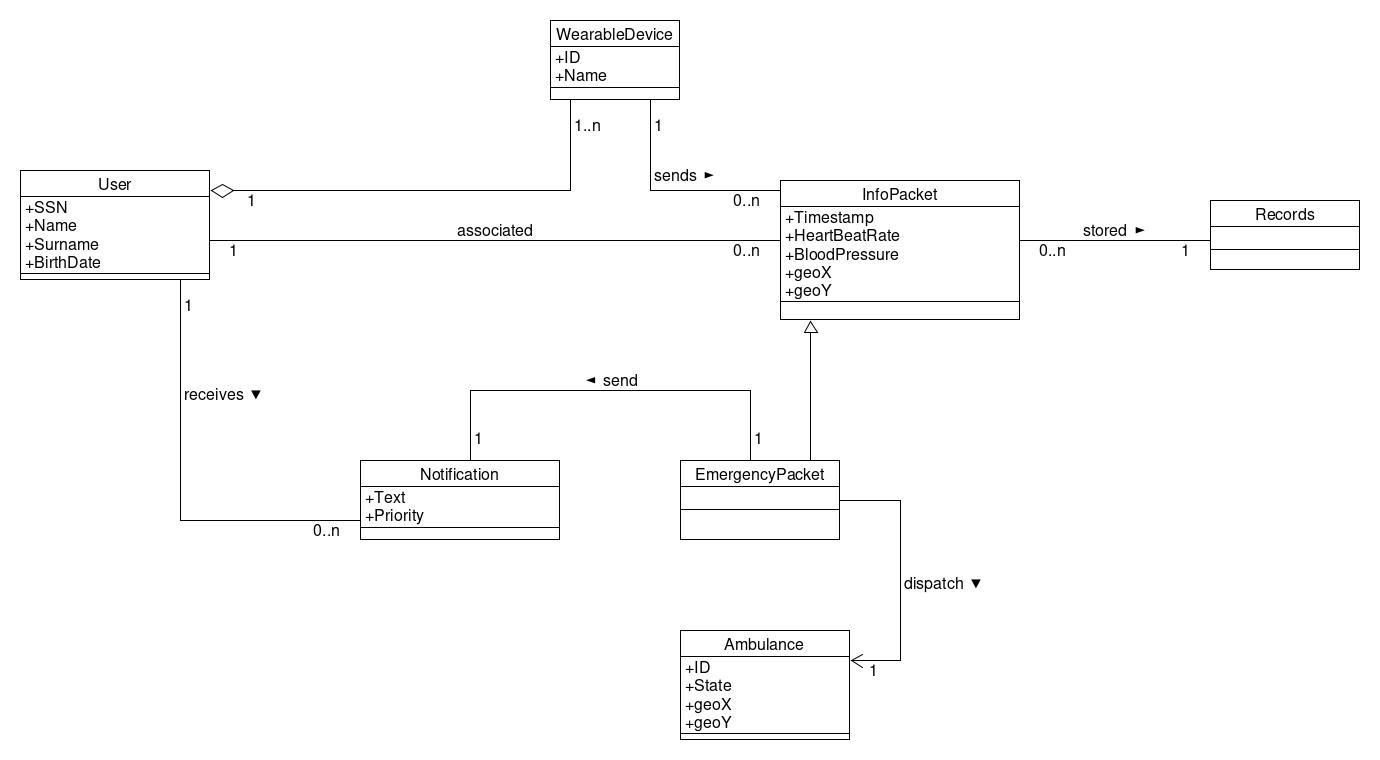
\includegraphics[width=\paperwidth, angle=90]{rasd_classdiag_sos.jpg}
	\caption{Class diagram for the AutomatedSOS service}
	\label{fig:classdiag_sos}
\end{figure}
\newpage
\thispagestyle{empty}
\begin{figure}[H]
	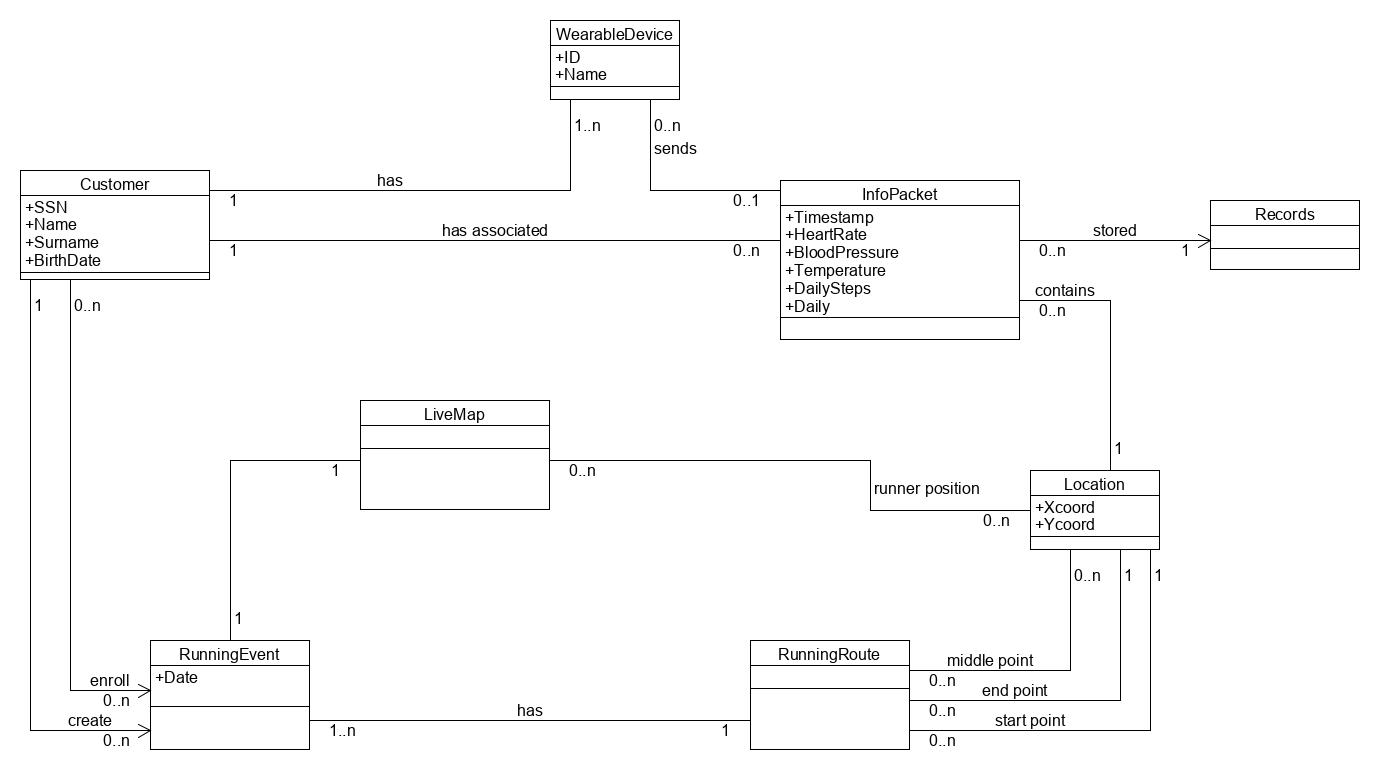
\includegraphics[width=\paperwidth, angle=90]{rasd_classdiag_t4r.jpg}
	\caption{Class diagram for the Track4Run service}
	\label{fig:classdiag_t4r}
\end{figure}
\newpage

\subsubsection{State machine diagrams}

Through the use of the state machine UML model, we desribe the evolution of the states for the main components of the system.

\begin{figure}[H]
	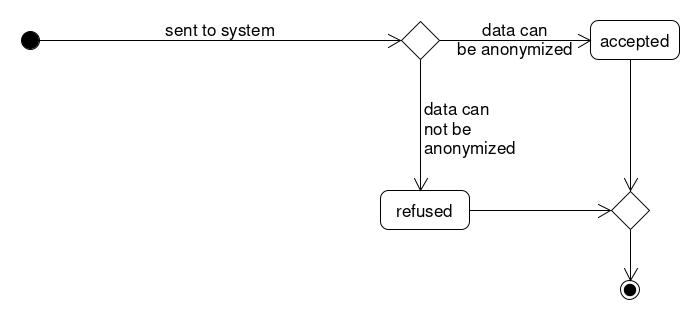
\includegraphics[width=\linewidth]{rasd_statemachine_grpreq.jpg}
	\caption{Statechart of a request for a group of cutsomers data}
	\label{fig:statemachine_grpreq}
\end{figure}

\begin{figure}[H]
	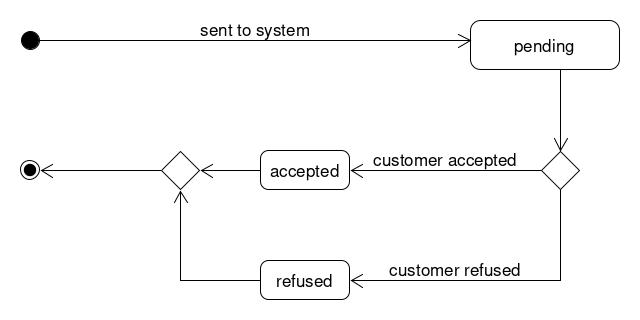
\includegraphics[width=\linewidth]{rasd_statemachine_specreq.jpg}
	\caption{Statechart of a request for a single cutsomer's data}
	\label{fig:statemachine_specreq}
\end{figure}

\begin{figure}[H]
	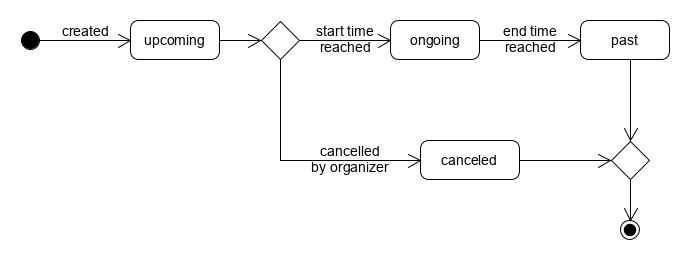
\includegraphics[width=\linewidth]{rasd_statemachine_runevent.jpg}
	\caption{Statechart of a running event}
	\label{fig:statemachine_runevent}
\end{figure}

\subsection{Product functions}

Following are the requirements our system has to satisfy in order to provide the main functionalities, each associated with its proper goal.

\begin{minipage}{\textwidth}
\vspace{4mm}
{\bf Data4Help}

\vspace{0.5cm}

\begin{description}
	\item [R1] The system must forward any request from a company to single customer's data to the corresponding user.
	\item \begin{flushright}{\bf{G1}}\end{flushright}

	\item [R2] The system must reject any request for data regarding a group of customers when it cannot guarantee the anonimity of its components.
	\item \begin{flushright}{\bf{G2}}\end{flushright}

	\item [R3] The system must periodically collect and store customer's data.
	\item \begin{flushright}{\bf{G3}}\end{flushright}

	\item [R3] The system must periodically collect and store customer's data.
	\item \begin{flushright}{\bf{G3}}\end{flushright}

	\item [R4] The system must periodically update the accessible data with the newly collected one
	\item \begin{flushright}{\bf{G4}}\end{flushright}

	\item [R5] The system must notify the user of the request and permit him to accept or refuse it.
	\item \begin{flushright}{\bf{G5}}\end{flushright}

	\item [R6] The system must update the request status with the answer provided by the user.
	\item \begin{flushright}{\bf{G5}}\end{flushright}

	\item [R7] The system must be able to identify which data can be accessed for each third party company.
	\item \begin{flushright}{\bf{G6}}\end{flushright}

\end{description}
\end{minipage}
\vspace{8mm}


\begin{minipage}{\textwidth}
{\bf AutomatedSOS}
\begin{description}
	\item [R8] The system must continuously check the data read from customers subscribed to AutomatedSOS.
	\item \begin{flushright}{\bf{G7}}\end{flushright}

	\item [R9] In case the data indicate an emergency for a customer, the system must dispatch the closest ambulance to his location.
	\item \begin{flushright}{\bf{G7}}\end{flushright}

	\item [R10] After an ambulance is dispatched, the system must notify the customer of its arrival.
	\item \begin{flushright}{\bf{G8}}\end{flushright}

\end{description}
\end{minipage}
\vspace{8mm}


\begin{minipage}{\textwidth}
{\bf Track4Run}
\begin{description}
	\item [R11] The system must allow users to define the route, the date and the time of the event.
	\item \begin{flushright}{\bf{G9}}\end{flushright}

	\item [R12] Two events can't overlap in the same place, date and time.
	\item \begin{flushright}{\bf{G9}}\end{flushright}

	\item [R13] The system must show open events to the users.
	\item \begin{flushright}{\bf{G10}}\end{flushright}

	\item [R14] The system must allow users to sort and filter events by date and location.
	\item \begin{flushright}{\bf{G10}}\end{flushright}

	\item [R15] The system must collect and provide in real time the position of participants on a map.
	\item \begin{flushright}{\bf{G11}}\end{flushright}

\end{description}
\end{minipage}
\vspace{8mm}

\subsection{User characteristics}
Following are the actors of the application:
\begin{itemize}
	\item Companies such as life insurances, hospitals and clinics, universities for research purposes or companies that focus on data analysis.
	\item People of any age in need for a potentially life saving system. They may have diseases, disabilities, or just be elder.
	\item Runners who want to organize running events or enroll in them, or people who want to track participants in real time.
	\item TrackMe's service staff, that will handle third parties registration and assist them in case of need, among other service activities.
\end{itemize}

\subsection{Assumptions, dependencies, constrains}

{\bf Domain assumptions}

\begin{description}

	\item [D1] Third parties are able to identify specific customers by SSN or FC.
	\item [D2] A group is considered anonymous if is composed by more than 1000 people.
	\item [D3] A sent request for customer's data is always received by the user.
	\item [D4] Health emergency status occurs when a AutomatedSOS customer parameters falls below of or exceeds healthy boundaries.
	\item [D5] AutomatedSOS customers always have an active and working internet connection.
	\item [D6] An ambulance is always available for dispatching and can reach the customer position.
	\item [D7] Organizers choose a valid path for a running event.
	\item [D8] A running event is legally autorized by the authorities.
	\item [D9] The user is supposed to be at least 18 years old.

\end{description}

\end{document}
